\documentclass[10pt,twocolumn,letterpaper]{article}

\usepackage{iccv}
\usepackage{times}
\usepackage{epsfig}
\usepackage{graphicx}
\usepackage{amsmath}
\usepackage{amssymb}
\usepackage{graphicx}

% ------ New Package Here ------
\usepackage{dblfloatfix}
\usepackage{subcaption}
\usepackage{bm}
\usepackage[pagebackref=true,breaklinks=true,letterpaper=true,colorlinks=true,bookmarks=true]{hyperref}
% ------------------------------

\makeatletter
\newcommand\footnoteref[1]{\protected@xdef\@thefnmark{\ref{#1}}\@footnotemark}
\makeatother


%---------MATH SYMBOLS NEW COMMANDS:--------------------------------------
\newcommand{\vectornorm}{|}

\newcommand{\diver}{\mathrm{div}}
\newcommand{\grad}{\mathrm{grad}}
\newcommand{\trace}{\mathrm{trace}}
\newcommand{\ud}{\mathrm{d}}

\newcommand{\mvec}[1]{\boldsymbol{#1}}
\newcommand{\matr}[1]{\mathrm{#1}}

\newcommand{\eye}{\mathrm{I}}
\newcommand{\img}{u}

\newcommand{\prob}[1]{\mathrm{p}\left( #1 \right)}

\newcommand{\bhat}{\widehat{\mvec{b}}}
\newcommand{\lamhat}{\widehat{\mvec{\lambda}}}
\newcommand{\eps}{\mvec{\varepsilon}}

%\newcommand{\norm}[1]{\left\Vert#1\right\Vert}
% \newcommand{\norm}[1]{\left \|#1 \right \|}
\newcommand{\norm}[1]{\left |#1 \right |}
\newcommand{\transp}{^\mathrm{T}}

\newcommand{\bu}{\boldsymbol{u}}
\newcommand{\bx}{\boldsymbol{x}}
\newcommand{\bp}{\boldsymbol{p}}

\newcommand{\be}{\boldsymbol{\varepsilon}}

\newcommand{\bv}{\boldsymbol{v}}
\newcommand{\mfsf}[0]{{\sc mfsf}}
\newcommand{\mfsfc}[0]{{\sc mfsf\em c}}
\newcommand{\mfsfdct}[0]{{\sc mfsf$_{\tt DCT}$}}
\newcommand{\mfsfpca}[0]{{\sc mfsf$_{\tt PCA}$}}
\newcommand{\mfsfid}[0]{{\sc mfsf$_{\tt I_{2F}}$}}
\newcommand{\mfsfcdct}[0]{{\sc mfsf\em c$_{\tt DCT}$}}
\newcommand{\mfsfcpca}[0]{{\sc mfsf\em c$_{\tt PCA}$}}
\newcommand{\mfsfcid}[0]{{\sc mfsf\em c$_{\tt I_{2F}}$}}


\newcommand{\cU}{\mathcal{U}}
\newcommand{\bU}{\boldsymbol{\mathcal{U}}}
\newcommand{\bE}{\boldsymbol{\mathcal{E}}}
\newcommand{\bI}{\boldsymbol{I}}
\newcommand{\bA}{\boldsymbol{A}}
\newcommand{\bb}{\boldsymbol{b}}
\DeclareMathOperator*{\argmin}{arg\,min}
\DeclareMathOperator*{\argmax}{arg\,max}


\newcommand{\bL}{\boldsymbol{L}}
\newcommand{\bM}{\boldsymbol{M}}

\newcommand{\R}{\mathbb{R}}

\newcommand{\Lone}{\mathbf{L}^1}
\newcommand{\Ltwo}{\mathbf{L}^2}


%----------------------------------------------------------------------------------------------------

% \iccvfinalcopy % *** Uncomment this line for the final submission

\def\iccvPaperID{1612} % *** Enter the ICCV Paper ID here
\def\httilde{\mbox{\tt\raisebox{-.5ex}{\symbol{126}}}}

% Pages are numbered in submission mode, and unnumbered in camera-ready
\ificcvfinal\pagestyle{empty}\fi

\begin{document}

%%%%%%%%% TITLE
\title{Supplementary Material: Constructing Statistical Deformable Models with Shape Flow}

\author{Yuxiang Zhou, Joan Alabort-i-Medina, Anastasios Roussos, Stefanos Zafeiriou\\
Imperial College London\\
180 Queen’s Gate, SW7 2AZ, London, U.K.\\
{\tt\small \{yuxiang.zhou10, ja310, troussos, s.zafeiriou\}@imperial.ac.uk}}
\maketitle
\thispagestyle{empty}


%%%%%%%%% Appendix
\appendix
\section{Introduction}
In this supplementary material, we provide additional experimental results and comparisons for the proposed pipeline of constructing dense AAMs without consistent set of landmarks. 
We present four different sets of experiments. 

reported to support applications of dAAMs. 

In Section \ref{sec:fittingresults}, we present visualisations of in-the-wild model fitting  for faces and ears, comparing classic AAMs and the proposed dense AAMs. In Section \ref{sec:modelanalysis}, we compares analytical qualities of our dAAMs with respect to that of classic aams in terms of model compactness, warping quality and reconstruction.
Moreover, experiment \ref{sec:reconstruct} serves as a qualitative demonstration of how the proposed pipeline can use be effectively used to generate novel modified instances of an object, e.g. caricatures, from simple hand drawn sketches.
Finally, experiment \ref{sec:segmentation} evaluates the effectiveness and performance of the proposed methodology to build dense AAMs of objects that are difficult to annotated with respect to a consistent set of landmarks, such as bottles and human bodies. Corresponding demonstration shows the usage of utilising dAAMs for objects segmentation.

\section{Fitting Results}
\label{sec:fittingresults}

This section provided additional visualisation results of experiments in original paper section 3.3 Non-rigid object alignment in-the-wild, where quantitative analysis of dense AAMs of ears and faces are shown. Although there are few figures demonstrated normalise point-to-point error measure of ear fitting, only sparse points are shown in order to maintain readability. But here we have visualisation of pixel-wise dense fitting results for both faces and ears. Results for this experiment of faces are reported over the 224 testing images of the LFPW database using 68 point ground truth landmark annotations
\footnote{\label{ibug_300} \url{http://ibug.doc.ic.ac.uk/resources/300-W/}}. 
For ears, we collected 605 high resolution images of ears in unconstrained scenarios and annotated them using both a newly defined 55 point annotation scheme for ears and the curve annotations proposed in the paper. Results for fitting ears are reported over 105 testing images.

Figure \ref{fig:fr} shows dense fitting results in grid view, thus dense points are visualisible without affecting the visibility of appearance. Full fitting results visualisation are provided in supplementary videos.

\begin{figure}[!t]
\centering
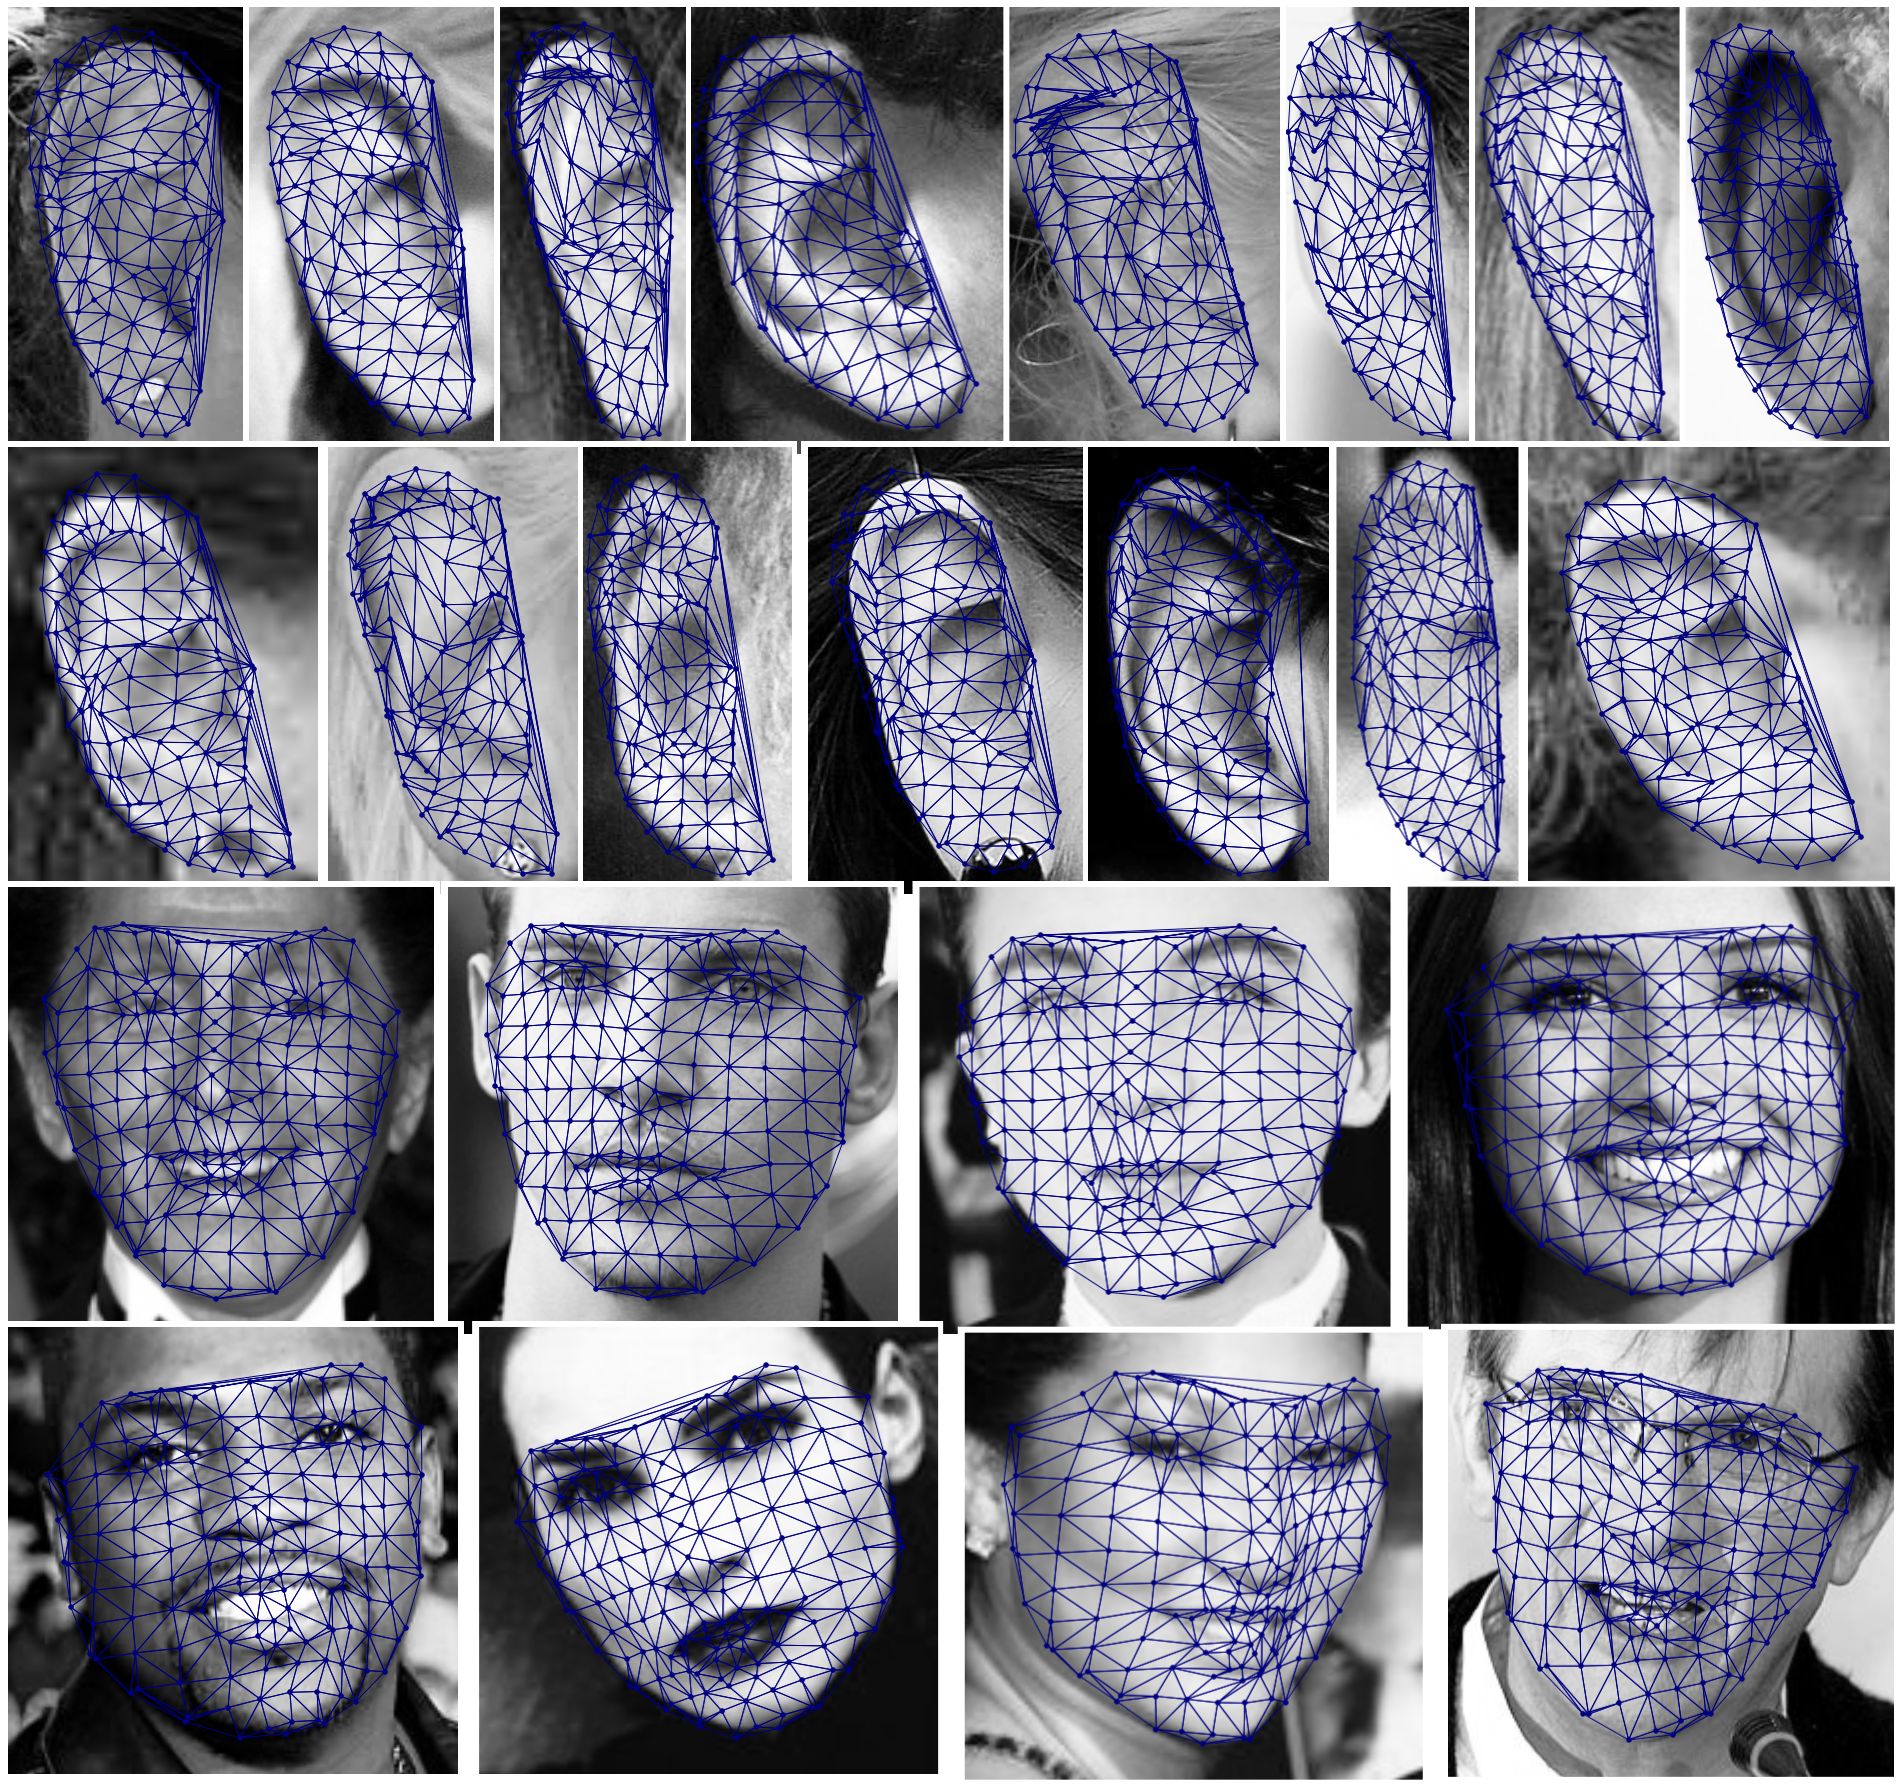
\includegraphics[width=0.45\textwidth]{supports/Fittings/fittings}
\caption{dAAMs Dense Grid Visualisation.}
\label{fig:fr}
\end{figure}

\section{Shape Models Analysis}
\label{sec:modelanalysis}

\begin{figure*}[!t]
\centering
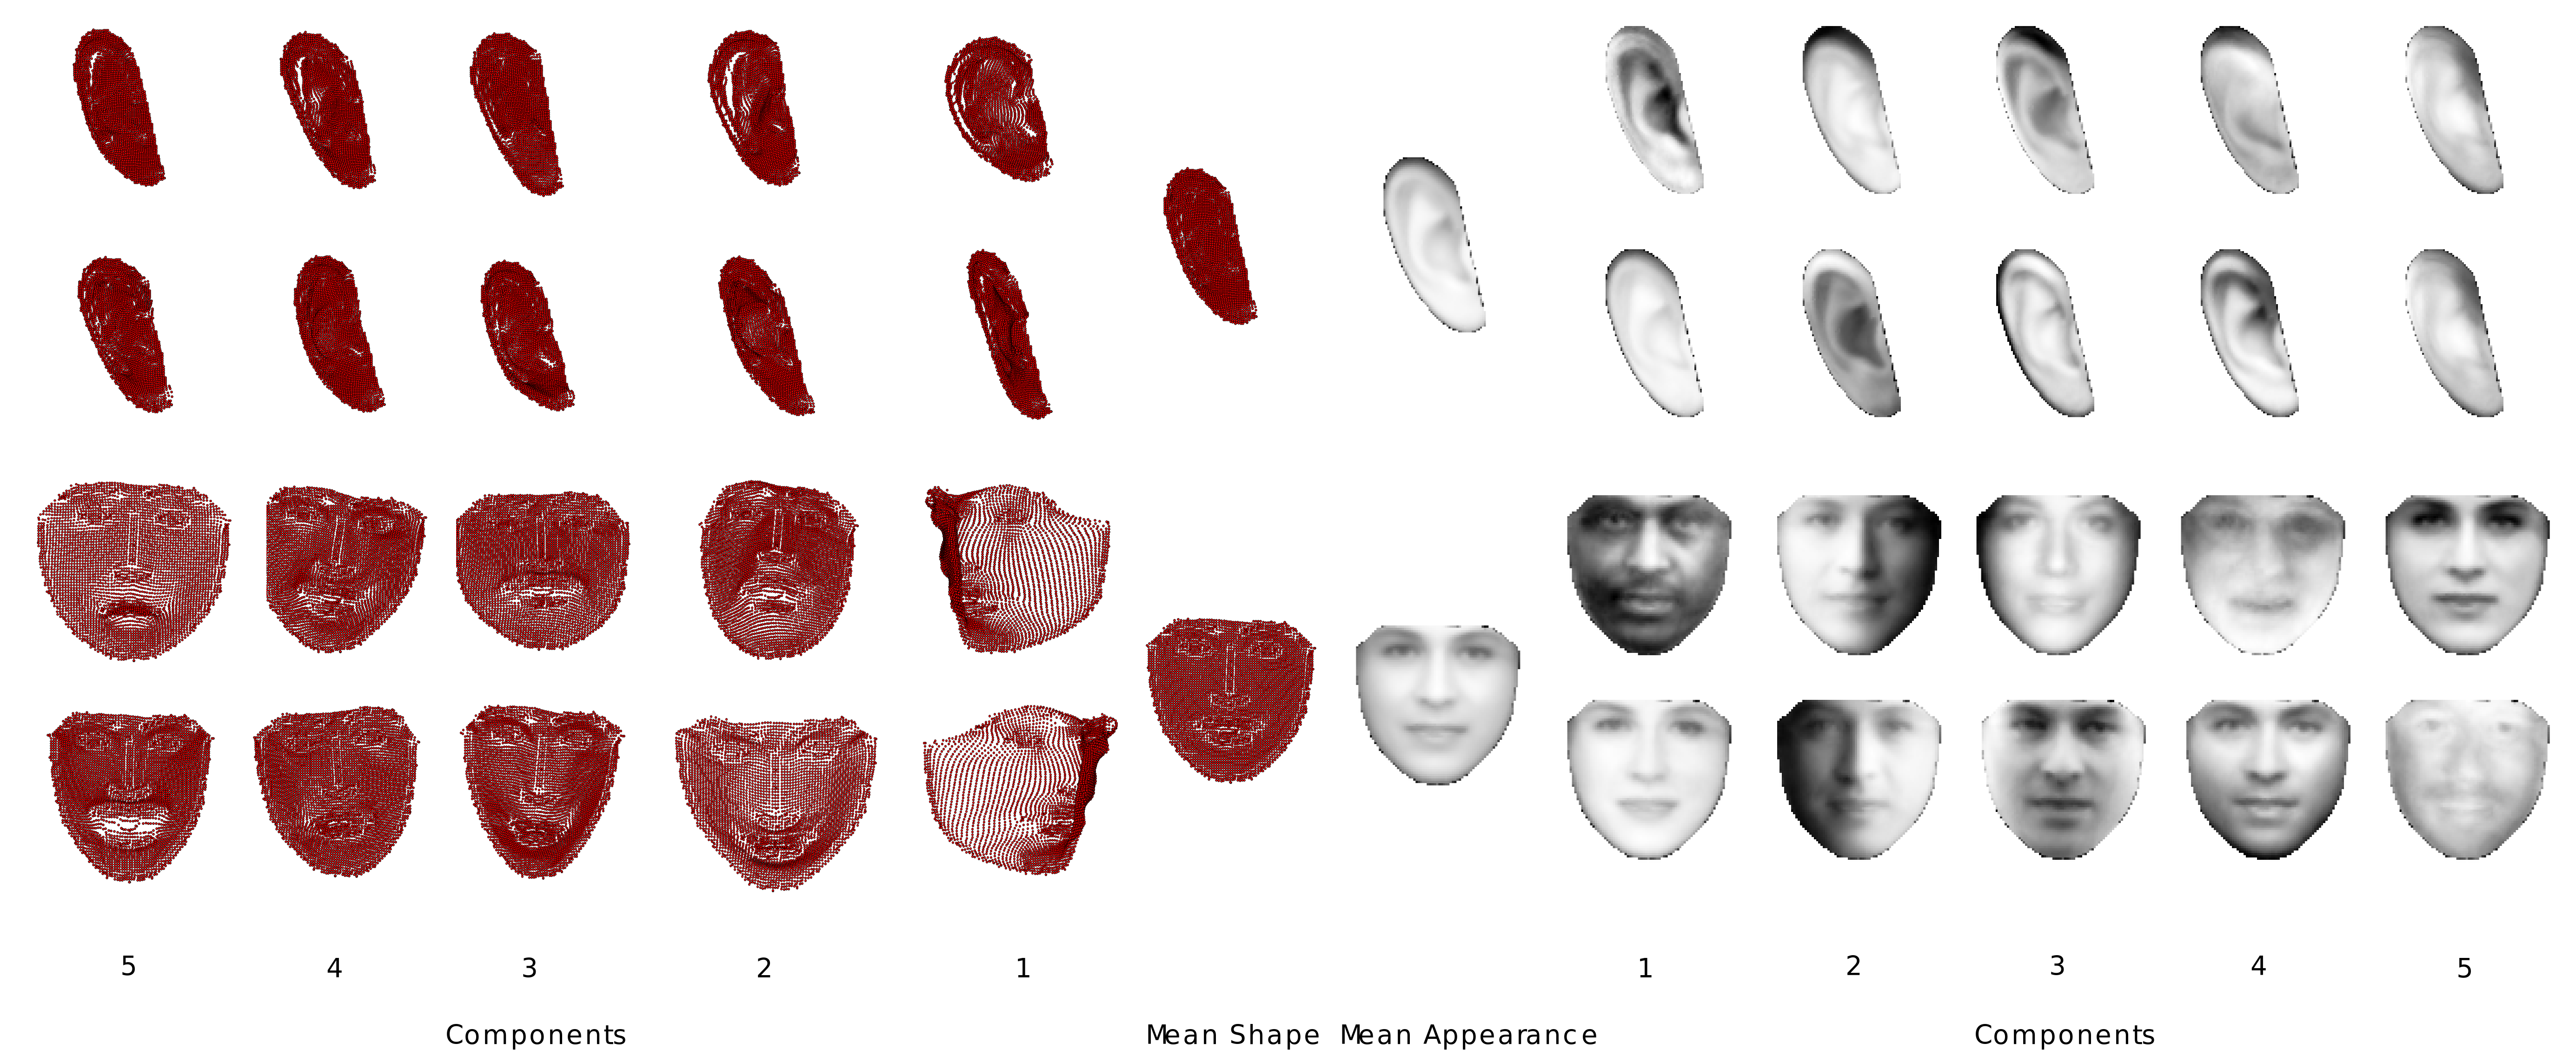
\includegraphics[width=\textwidth]{supports/Models/models}
\caption{First Five Principle Components Visualisation of dAAMs on Ears and Faces}
\label{fig:pcamodel}
\end{figure*}

There are two experiments shown in this section. First experiment investigate the impact of constructing dense points correspondence. Note that we are using the same AAMs and dAAMs models built from experiments \ref{sec:fittingresults}. The experiment is used to reveal accuracy of dense model reconstruction in shape space. In particular, given a ground-truth shape, we use shape models from both AAMs and dAAMs to reconstruct the given shape densely. As AAMs having sparse shape model, we densify it the same way as warping textures on to shape model, in this case is piecewise affine transform. 

\begin{figure}[!b]
    \centering
    \vspace*{-0.1in}
    \begin{subfigure}[b]{0.4\textwidth}
            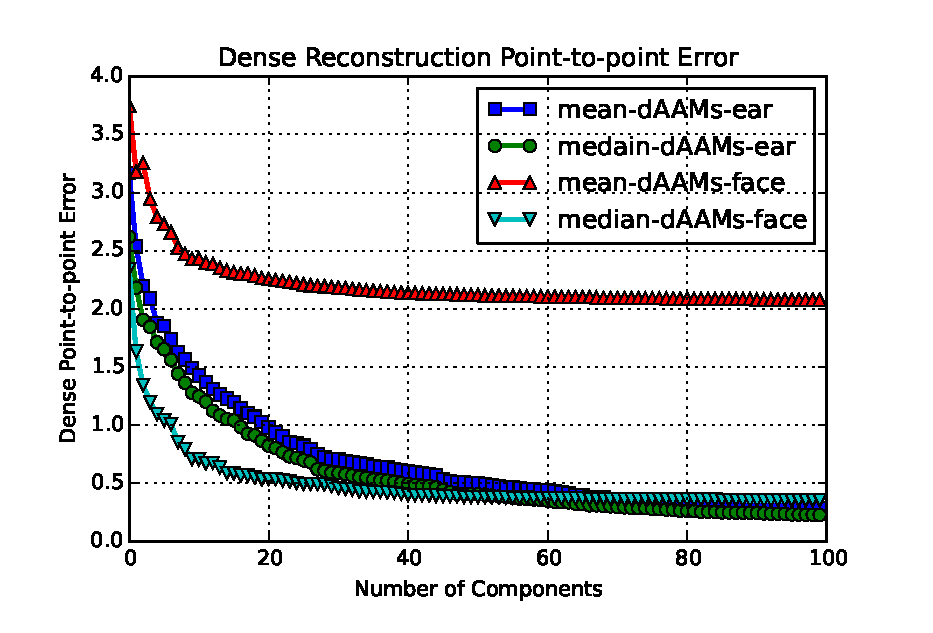
\includegraphics[width=\textwidth]{supports/Model_Analysis/sr_daams}
        %\caption{dAAMs dense shape reconstruction}
    \end{subfigure}
    \\
    \begin{subfigure}[b]{0.4\textwidth}
            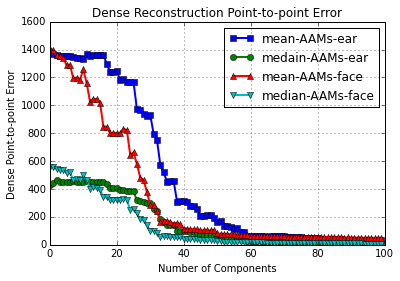
\includegraphics[width=\textwidth]{supports/Model_Analysis/sr_aams}
        %\caption{AAMs dense shape reconstruction}
    \end{subfigure}
    \caption{Dense Shape Reconstruction}
    \label{fig:rc_face}
\end{figure}

Statistical evaluation are given in terms of the normalised point-to-point error measure for reconstructing both ears and faces. Figure \ref{fig:rc_face} clearly shows the number of shape components used for reconstruction and corresponding normalised point-to-point error in terms of mean and variance. It manifests dAAMs is significantly out performed classic AAMs on shape reconstruction. The reconstruction of appearance are shown in experiment \ref{sec:reconstruct}.

\begin{figure}[!b]
    \centering
    \includegraphics[width=0.45\textwidth]{resources/Fig_Draw/draw}
    \caption{Caricatures Appearance Reconstruction}
    \label{fig:draw}
\end{figure}

Second experiment are performed to investigate the impact of shape components of AAMs and dAAMs in terms of variance ratio of eigenvalues, shown in figure \ref{fig:compact}. We can observe in detail variance ratio of each principle components of shape models and cumulative ratio of first few components. As plot revealed, dAAMs proved having a more compact shape model as first few components captures higher variance ratio than that of classic AAMs, therefore less components are needed in order to capture certain amount of variance which leads to better reconstruction especially with few shape components.

Figure \ref{fig:pcamodel} demonstrated shape and appearance models visualisation for dense AAMs of ears and faces. Middle column shows mean shape and mean appearance while rest columns present corresponding principle components with $\pm 3$ variance.

\begin{figure}[!t]
    \centering
    \begin{subfigure}[b]{0.4\textwidth}
            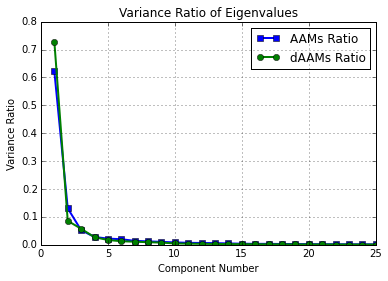
\includegraphics[width=\textwidth]{supports/Model_Analysis/variance_ratio}
        %\caption{dAAMs vs AAMs Variance Ratio}
    \end{subfigure}
    \begin{subfigure}[b]{0.4\textwidth}
            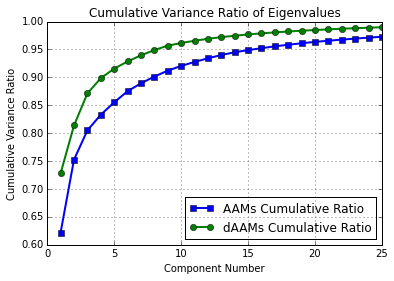
\includegraphics[width=\textwidth]{supports/Model_Analysis/cumulative_variance_ratio}
        %\caption{dAAMs vs AAMs Cumulative Variance Ratio}
    \end{subfigure}
    \caption{dAAMs vs AAMs Variance Ratios}
    \label{fig:compact}
\end{figure}

\section{Appearance Reconstruction}
\label{sec:reconstruct}

\begin{table}[!b]
\small
\centering
\begin{tabular}{|l|c|c|c|}
\hline
\emph{Object}   & \emph{mean} & \emph{std} & \emph{median}\\
\hline\hline
Bottles         & 0.8125      & 0.1460     & 0.8414\\
Action - Jump   & 0.6102      & 0.0198     & 0.6099\\
Action - Slide  & 0.6444      & 0.0500     & 0.6501\\
\hline
\end{tabular}
\caption{Segmentation statistics for experiment \ref{sec:segmentation}}
\label{tab:seg_result}
\end{table}

This experiment serves as a qualitative demonstration of how the proposed pipeline can be effectively used to generate novel modified instances of an object, e.g. caricatures. To be specific, firstly we manually craft a set of hand-drawn cartoon-like shape sketch before applying shape flow on them to align with reference frame, thus having dense correspondence of landmarks. Following with shape reconstruction using both AAMs and dAAMs. Lastly warp appearance from arbitrarily chosen faces onto reconstructed shape using piecewise affine (of AAMs) and shape flow (of dAAMs). 

The comprehensive results are shown in figure \ref{fig:draw}, where first column is caricatures, second is source textures, third and last columns are corresponding reconstructions of AAMs and dAAMs. Comparing with dAAMs, AAMs turned to introduce artifacts on reconstructions especially mouth and eyes area, where nuanced information are missing or models are overly deformed. Again, dAAMs not only have remarkable non-rigid alignment performance against AAMs (experiment \ref{sec:fittingresults}) but performs considerably better at objects reconstruction.

\section{Segmentation using Dense AAM}
\label{sec:segmentation}

\begin{figure}[!t]
    \centering
    \begin{subfigure}[b]{0.15\textwidth}
            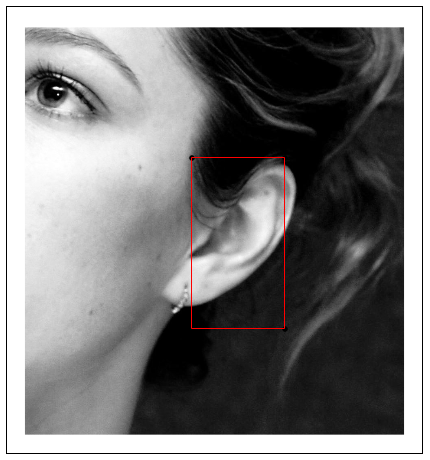
\includegraphics[height=\textwidth]{supports/Segmentation_Measure/ear}
        %\caption{Ear Initial Bounding Box}
    \end{subfigure}
    \begin{subfigure}[b]{0.15\textwidth}
            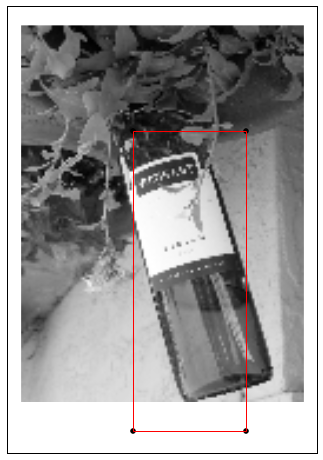
\includegraphics[height=\textwidth]{supports/Segmentation_Measure/bottle}
        %\caption{Bottle Initial Bounding Box}
    \end{subfigure}
    \begin{subfigure}[b]{0.15\textwidth}
            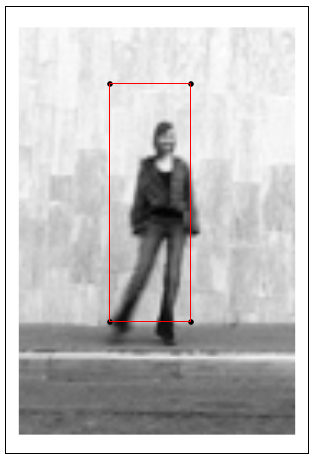
\includegraphics[height=\textwidth]{supports/Segmentation_Measure/body}
        %\caption{Body Initial Bounding Box}
    \end{subfigure}
    \caption{Perturb Initialisation of Object Detector}
    \label{fig:seg_init}
\end{figure}

In this section, we experimenting on utilising our dense AAM for objects segmentation. Two subjects, bottles and human, are involved. As for human segmentation, we gather ground true images from Space-Time Actions
\footnote{\label{sta} \url{http://www.wisdom.weizmann.ac.il/~vision/SpaceTimeActions.html}},
where several human action sequences are provided with segmentation. There are 10 categories actions where each category contains 10 subjects each are recorded with more than 120 frames. For bottles, 500 high resolution images of bottles are collected and annotated using not only a newly defined 50 point annotation scheme for bottles, but also the curve annotations proposed in this paper. We randomly split the previous database into two disjoint sets of training (400) and testing (100) images. Bottle models were built using 400 training images while body models are built in terms of human actions (e.g. jumping), each having approximately 200 training images and 50 test images. Note here that we used the same procedures used in experiment \ref{sec:fittingresults} to build models. 

Fitting dAAMs on test images gives dense landmarks which could be used to perform segmentation. A simple object detector would be required in prior to our pipeline to initialise the fitting. For simple evaluation, we perturb the ground-truth segmentation with certain variance to simulate an object detector with implicit detection. Initialisation samples are shown in Figure \ref{fig:seg_init}. The performance of fitting bottles and bodies are measured based on the segmentation precision shown in Table \ref{tab:seg_result}, where statistical results including mean, variance and median are presented.
    
{\small
\bibliographystyle{ieee}
\bibliography{bib}
}

\end{document}